\documentclass{beamer}
\mode<presentation>
\usepackage[utf8]{inputenc}
\usepackage{algorithm,algorithmicx,amssymb,amsmath,amsthm,bbm,color,epstopdf,float,geometry,graphicx,hyperref,listings,mathrsfs,mathtools,multirow,subcaption,textgreek,xcolor}

\usepackage[noend]{algpseudocode}
\usepackage{algcompatible}



\usepackage{float}
\renewcommand{\algorithmicrequire}{\textbf{Input:}}
\renewcommand{\algorithmicensure}{\textbf{Output:}}
    
% \usepackage[linesnumbered,ruled,vlined]{algorithm2e}
\usepackage[flushleft]{threeparttable}
\usepackage[shortlabels]{enumitem}
\usepackage[table]{xcolor}
\newcommand{\JLcolor}[1]{{\textcolor{violet}{#1}}} %violet

% Create Background Pic
%\usepackage{tikz}
%\definecolor{bottomcolour}{rgb}{0.32,0.3,0.38}
%\definecolor{topcolour}{rgb}{0.08,0.08,0.16}
%\setbeamertemplate{background canvas}{%
%	\begin{tikzpicture}[remember picture,overlay]
%	\shade[top color=topcolour,bottom color=bottomcolour]
%(current page.north west) rectangle (current page.south east);
%	\end{tikzpicture}%     
%}


%=======================================================
% Set page number
\setbeamertemplate{footline}[page number]

%=======================================================
%\usetheme{Boadilla}
\setbeamerfont{title}{size=\fontsize{18pt}{18pt}\selectfont} % bold font: \bfseries
\setbeamerfont{author}{size=\fontsize{20pt}{20pt}\selectfont}
\setbeamerfont{institute}{size=\fontsize{13pt}{13pt}\selectfont}
%\setbeamercolor{itemize item}{fg=red}

%================================================
%Set font color
\definecolor{mygray1}{rgb}{0.7421875,0.7421875,0.7421875}
\definecolor{mygray2}{gray}{0.6}
\definecolor{mygray3}{rgb}{0.55, 0.52, 0.54}
\definecolor{mybrown1}{rgb}{0.28, 0.24, 0.2}
\definecolor{myred}{rgb}{0.68, 0.09, 0.13}
\definecolor{myginger}{rgb}{0.69, 0.4, 0.0}
\definecolor{myblue1}{rgb}{0.0, 0.2, 0.6}
\definecolor{myblue2}{rgb}{0.38, 0.51, 0.71}
\definecolor{myblue3}{rgb}{0.2,0.2,0.7}
\definecolor{mygreen}{rgb}{0.42, 0.56, 0.14}
\definecolor{myviolet}{rgb}{0.54, 0.17, 0.89}


\newcommand{\highlightA}[1]{\colorbox{myblue3!50!}{$\displaystyle #1$}}
\newcommand{\highlightB}[1]{\colorbox{myred!50!}{$\displaystyle #1$}}
\newcommand{\highlightC}[1]{\colorbox{mygreen!50!}{$\displaystyle #1$}}
%================================================
% set picture source
\usepackage[absolute,overlay]{textpos}

\setbeamercolor{framesource}{fg=gray}
\setbeamerfont{framesource}{size=\tiny}
\newcommand{\source}[1]{\begin{textblock*}{4cm}(8.7cm,8.6cm)
\begin{beamercolorbox}[ht=0.5cm,right]{framesource}
\usebeamerfont{framesource}\usebeamercolor[fg]{framesource} Source: {#1}
\end{beamercolorbox}
\end{textblock*}}

\setbeamercolor{frametitle}{fg=white,bg=black}


%================================================
% url color
\renewcommand\UrlFont{\color{myblue3}}
%================================================

\newtheorem{Thm}{{\bf Theorem}}


% Make first page
\makeatletter
\setbeamertemplate{navigation symbols}{}
\title[MFMC for Tokamak UQ]{Iterative Integer-Valued Sample Size \\Allocation for Multi-Fidelity Monte Carlo}
%\subtitle[short version]{}
\date{\today\\[2em]
{\footnotesize Partially supported by the U. S. Air Force Research Laboratory through the grant AFOSR FA9550-22-1-0004. }
}

\author[J.Liang]{\normalsize  Jiaxing Liang\\ }
\institute[Rice University]{\fontsize{8}{8} Department of Computational Applied Mathematics \& Operations Research, Rice University}




%=======================================================
\begin{document}
\frame{\titlepage }

% %=======================================================
% \begin{frame}{Motivation}
% \begin{itemize}
% \item Multi-fidelity Monte Carlo (MFMC) combines expensive high-fidelity models with cheaper low-fidelity approximations
% \item \textbf{Challenge}: Continuous optimal allocations require integer sample sizes in practice
% \item \textbf{Problem}: Direct flooring leads to:
% \begin{itemize}
% \item Budget under-utilization 
% \item Degenerate estimators (infinite variance)
% \item Suboptimal variance performance
% \end{itemize}
% \end{itemize}
% \end{frame}




%=======================================================
\begin{frame}[t]
\frametitle{Multi-fidelity Monte Carlo}
\begin{itemize}[leftmargin=5pt] 

    \item[$\triangleright$] \textcolor{myblue3}{\bf Computational Challenges in UQ}
    \begin{itemize}[leftmargin=15pt] 
    \item[$\circ$] High-fidelity models are \textbf{computationally expensive}
    \item[$\circ$] Traditional Monte Carlo requires \textbf{many samples}
    \item[$\circ$] \textbf{Multi-fidelity approaches} combine models of varying accuracy/cost
    \end{itemize}
    
    \item[$\triangleright$] \textcolor{myblue3}{\bf Framework: Multi-fidelity Monte Carlo (MFMC)} 
    \begin{itemize}[leftmargin=15pt] 
    \item[$\circ$] \textbf{High-fidelity (HF)}: Expensive but accurate
    \item[$\circ$] \textbf{Low-fidelity (LF)}: Cheap but less accurate
    \item[$\circ$] \textbf{Key insight}: Leverage correlations between models
    \item[$\circ$] \textbf{Goal}: Minimize estimator variance under fixed budget
    \end{itemize}   
    %
    \vspace{1mm}
    %
    {\fontsize{8}{8}\selectfont \textcolor{mygray2}{B. Peherstorfer, K. Willcox, and M. Gunzburger. Optimal Model Management for Multifidelity Monte Carlo Estimation. SIAM J. SCI. COMPUT, Vol. 38, No. 5, pp. A3163–A3194.}\par}
    
    \item[$\triangleright$] \textcolor{myblue3}{\bf The Sampling Dilemma}
    \begin{itemize}[leftmargin=15pt] 
    \item[$\circ$] How many samples from each model?
    \item[$\circ$] How to balance \textbf{accuracy vs. computational cost}?
    \item[$\circ$] How to handle \textbf{integer sample sizes} in practice?
    \end{itemize}
    
\end{itemize}
\end{frame}




% ====================================================
\begin{frame}{MFMC Estimator Construction}
\begin{itemize}[leftmargin=5pt] 

    \item[$\triangleright$] \textcolor{myblue3}{\bf Models:} 
    \[
    u_1 \;\; \text{(HF)}, \quad u_k\;\; \text{(LF)},\quad  k=2,\dots,K.
    \]
    \item[$\triangleright$]\textcolor{myblue3}{\bf MFMC estimator $A^{\text{MF}}$ for $\mathbb{E}[u]$:} 
    
\[
\boxed{
A^{\text{MF}} := A^{\text{MC}}_{1,N_1} + \sum_{k=2}^K \alpha_k\big(\overline{A}_{k,N_k} - \overline{A}_{k,N_{k-1}}\big)
}
\]
\begin{itemize}[leftmargin=15pt] 
  \item[$\circ$] $A^{\text{MC}}_{1,N_1}$: Monte Carlo estimator using $N_1$ HF samples.
  \item[$\circ$] $\alpha_k$: control variate weights.
  \item[$\circ$] $\overline{A}_{k,N_{k-1}}$ reuses the first $N_{k-1}$ samples from $\overline{A}_{k,N_{k}}$. 
  
  Nested sampling condition: $N_{k-1}\le N_k$.
  \item[$\circ$] Unbiased $\mathbb{E}[A^{\text{MF}}] = \mathbb{E}[u_h]$.
\end{itemize}
% \vspace{1em}
\item[$\triangleright$] \textcolor{myblue3}{\bf Variance functional:} 
\[
\boxed{
\mathcal{V}^{\text{MF}}(\alpha_k, N_k)
    =\frac{\sigma_1^2}{N_1} 
    + \sum_{k=2}^K \!\Big(\frac{1}{N_{k-1}} - \frac{1}{N_k}\Big)\!
      \big(\alpha_k^2\sigma_k^2 - 2\alpha_k\rho_{1,k}\sigma_1\sigma_k\big)
}
\]
\end{itemize}
\end{frame}



% ====================================================
\begin{frame}{Optimal Weights \& Simplified Variance }
\begin{itemize}[leftmargin=5pt] 

\item[$\triangleright$] \textcolor{myblue3}{\bf Variance:}
    {\footnotesize
    \[
    \mathcal{V}^{\text{MF}}(\alpha_k, N_k)
    =\frac{\sigma_1^2}{N_1} 
    + \sum_{k=2}^K \!\Big(\frac{1}{N_{k-1}} - \frac{1}{N_k}\Big)\!
    \big(\alpha_k^2\sigma_k^2 - 2\alpha_k\rho_{1,k}\sigma_1\sigma_k\big)
    \]
    }

\item[$\triangleright$] \textcolor{myblue3}{\bf Optimization Problem:}
    {\footnotesize
    \[
    \min_{\alpha_k,N_k}\mathcal{V}^{\text{MF}} \quad
    \text{s.t. } \sum_{k=1}^K C_k N_k = p, \;
    N_{k-1}\le N_k, \; N_k\ge 0
    \]
    \[
    C_k = \text{cost per sample}, \quad p = \text{total budget.}
    \]
    }
    
\item[$\triangleright$] \textcolor{myblue3}{\bf Optimal Weights:} 
{\footnotesize
The minimization over $\alpha_k$ is separable and convex:
    \[
    \alpha_k^* = \frac{\rho_{1,k}\sigma_1}{\sigma_k}
    \]
    }
    
\item[$\triangleright$] \textcolor{myblue3}{\bf Simplified Variance:}
{\footnotesize
    \[
    \mathcal{V}^{\text{MF}}(\alpha_k^*,N_k)
    = \sigma_1^2\sum_{k=1}^K \frac{\Delta_k}{N_k},
    \quad
    \Delta_k = \rho_{1,k}^2 - \rho_{1,k+1}^2,\;\rho_{1,K+1}=0
    \]
    \textcolor{myred}{\bf \normalsize Remark:} Define $\displaystyle f(N_k)=\sum_{k=1}^K\frac{\Delta_k}{N_k}$, Minimize $f(N_k)$ under cost constraint.
    }
\end{itemize}
\end{frame}


% ====================================================
\begin{frame}[t]
    \frametitle{Continuous Optimization Problem}
    % {\footnotesize Let $\Delta_k = \rho_{1,k}^2 - \rho_{1,k+1}^2$ for $k = 1, \dots, K$, with $\rho_{1,K+1} = 0$.}
    \begin{itemize}[leftmargin=5pt] 
     \vspace{3mm}
        \item \textcolor{myblue3}{\bf Original Formulation}
        {\footnotesize
                %
        \begin{equation*}\label{eq:Optimization_pb_sample_size}
            \begin{array}{ll}
            \min &\mathcal{V}^{\text{MF}}(\alpha_k, N_k),\\
               \text{subject to} &\displaystyle\sum\limits_{k=1}^K C_kN_k=p,\\[2pt]
               &\displaystyle -N_1\le 0,\quad \displaystyle N_{k-1}-N_k\le 0, \;\; k=2\ldots,K,\\
               &N_1,\ldots, N_K\in \mathbb{R},\\
               &\alpha_2,\ldots,\alpha_K\in \mathbb{R}.
            \end{array}
        \end{equation*}
        %
        }

        \item \textcolor{myblue3}{\bf  Reduced formulation}
        {\footnotesize
                %
        \begin{equation*}\label{eq:Optimization_pb_sample_size}
            \begin{array}{ll}
            \min &\displaystyle\sum_{k=1}^K \frac{\Delta_k}{N_k},\\
            \text{subject to} &\displaystyle\sum\limits_{k=1}^K C_kN_k=p,\\[2pt]
               &\displaystyle -N_1\le 0,\quad \displaystyle N_{k-1}-N_k\le 0, \;\; k=2\ldots,K,\\
               &N_1,\ldots, N_K\in \mathbb{R}.
            \end{array}
        \end{equation*}
        }
        
    \end{itemize}
\end{frame}




% ====================================================
\begin{frame}[t]
    \frametitle{MFMC Optimal Sample Allocation {\small [Peherstorfer et al. 2016]}}
    % \begin{itemize}[leftmargin=5pt] 
    %  \vspace{3mm}
    %     \item[$\triangleright$] The original optimization problem
        {\fontsize{8}{8}\selectfont 
        %
        % \begin{theorem}[Original problem -- Constraint on budget]
        % \label{thm:Sample_size_est}
        \textcolor{myblue3}{\bf \normalsize Given:}
        \begin{itemize}[leftmargin=15pt] 
            \item[$\circ$] $K$ models with variance $\sigma_k$, correlation $\rho_{1,k}$, and cost $C_k$
            \item[$\circ$] Total cost $p$
            \item[$\circ$] Define $\Delta_k = \rho_{1,k}^2 - \rho_{1,k+1}^2, \;\rho_{1,K+1}=0$
        \end{itemize}

        \textcolor{myblue3}{\bf \normalsize Assumption:}
        \begin{itemize}[leftmargin=15pt] 
            \item[$\circ$] Monotonic correlation: $|\rho_{1,1}| > \cdots > |\rho_{1,K}|$
            \item[$\circ$] Cost–correlation ratio: $\frac{\Delta_{k}}{C_k} > \frac{\Delta_{k-1}}{C_{k-1}}$
        \end{itemize}

        \vspace{5mm}

        
        \textcolor{myblue3}{\bf \normalsize Solution:}
        \begin{itemize}[leftmargin=15pt] 
            \item[$\circ$] Optimal weights: $\alpha_k^* = \dfrac{\rho_{1,k}\sigma_1}{\sigma_k}$
            \item[$\circ$] Optimal sample sizes:
            \[
        N_k^* = \sqrt{\frac{\Delta_k}{C_k}}\frac{p}{\sum_{j=1}^K \sqrt{C_j\Delta_j}}
        \] 
            \item[$\circ$] Optimal variance:
            %
        \begin{equation*}
        \label{eq:MFMC_variance_optimal}
        \mathcal{V}^{\text{MF}}_{\min} =
        % \frac{\sigma_1^2}{N_1^*} - \sum_{k=2}^K \left(\frac{1}{N_{k-1}^*} - \frac{1}{N_k^*}\right)\rho_{1,k}^2\sigma_1^2=
        \frac{\sigma_1^2}{p}\left(\sum_{k=1}^K\sqrt{C_k\Delta_{k}}\right)^2
        \end{equation*}
        %
        \end{itemize}
        
        % \end{theorem}
        }

\end{frame}


% ====================================================
\begin{frame}{Integer Allocation in Practice -- Direct Flooring }

\begin{itemize}[leftmargin=5pt] 
% \vspace{3mm}
\item[$\triangleright$] Real-valued $N_k^*$ must be rounded: \textcolor{myblue3}{\bf Direct Flooring}
{\footnotesize
\[
\lfloor N_k^* \rfloor = \text{floor}\left(\sqrt{\frac{\Delta_k}{C_k}} \frac{p}{\sum_{j=1}^K \sqrt{C_j \Delta_j}}\right)
\]

\[
N_k^* -1\le \lfloor N_k^*\rfloor \le N_k^*
\]
\begin{align*}
&\textbf{Budget bounds:}\qquad \mathcal{W}^{\text{MF}}(\lfloor N_k^* \rfloor) \in \left(p - \sum_{k=1}^K C_k, p\right] \\
&\textbf{Variance bounds:} \qquad f(\lfloor N_k^* \rfloor) \in \left[f(N_k^*), f(N_k^*-1)\right)=\left[\sum_{k=1}^K\frac{\Delta_k}{N_k^*},
\sum_{k=1}^K\frac{\Delta_k}{N_k^*-1}\right)
\end{align*}
}


\item[$\triangleright$] \textcolor{myblue3}{\bf Interpretation}
{\footnotesize
\begin{itemize}[leftmargin=15pt] 
\item[$\circ$] Cost slack: $\sum C_k$ (can be substantial for expensive models)
\item[$\circ$] Variance penalty: Bounded but can be significant
\item[$\circ$] Asymptotically negligible as $p \to \infty$, but problematic for moderate budgets
\end{itemize}
}
\end{itemize}
\end{frame}

% ====================================================
\begin{frame}{Rounding Effects}
\begin{itemize}[leftmargin=5pt] 
\item[$\triangleright$] \textcolor{myblue3}{\bf Continuous Optimal Solution}
\[
N_k^* = \sqrt{\frac{\Delta_k}{C_k}} \frac{p}{\sum_{j=1}^K \sqrt{C_j \Delta_j}}
\]
\item[$\triangleright$] \textcolor{myblue3}{\bf Direct Flooring $\lfloor N_k^*\rfloor$ Issues}

\textit{Rounding-induced slack is asymptotically negligible,}
but in the pre-asymptotic regime, budget under-utilization can be nontrivial.

\begin{itemize}[leftmargin=15pt] 
\item[$\circ$] \textbf{Budget underutilization}: $\sum C_k \lfloor N_k^* \rfloor \le p$
\item[$\circ$] \textbf{Degenerate estimators}: $\lfloor N_k^* \rfloor = 0$ for high-cost models
\item[$\circ$] \textbf{Variance inflation}: $f(\lfloor N_k^* \rfloor) \ge f(N_k^*)$
\item[$\circ$] \textbf{Suboptimal performance}: Independent rounding ignores budget redistribution
\end{itemize}
% \item[$\triangleright$] \textcolor{myred}{\bf Research Question:}

% Can we construct integer allocations that minimize budget slack while maintaining optimal variance properties?
\end{itemize}
\end{frame}

% ===========================================================
\begin{frame}{Research Questions}
\begin{itemize}[leftmargin=5pt] 
\item \textcolor{myred}{\bf Main Research Question}

Can we construct integer-valued sample size allocations that:
\begin{itemize}[leftmargin=15pt] 
\item[$\circ$] Minimize budget underutilization?
\item[$\circ$] Prevent degenerate estimators?
\item[$\circ$] Achieve better variance performance than direct flooring?
\item[$\circ$] Maintain theoretical guarantees?
\end{itemize}

\vspace{1em}
\item \textcolor{myblue3}{\bf Our Approach}
\begin{itemize}[leftmargin=15pt] 
\item[$\circ$] Dynamic programming formulation using Bellman's principle
\item[$\circ$] Iterative allocation with budget updates
\item[$\circ$] Minimum sample enforcement for robustness
\item[$\circ$] Theoretical analysis of cost and variance bounds
\end{itemize}
\end{itemize}
\end{frame}


% ========== SECTION 4: METHODOLOGY ==========
% ===========================================================
\begin{frame}{Problem Revisit \& Observation}
\begin{itemize}[leftmargin=5pt] 
\item[$\triangleright$] \textcolor{myblue3}{\bf Reduced continuous optimization problem}
{\footnotesize
        \begin{equation*}\label{eq:Optimization_pb_sample_size}
            \begin{array}{ll}
            \min &\displaystyle\sum_{k=1}^K \frac{\Delta_k}{N_k},\\
            \text{subject to} &\displaystyle\sum\limits_{k=1}^K C_kN_k=p,\\[2pt]
               &\displaystyle -N_1\le 0,\quad \displaystyle N_{k-1}-N_k\le 0, \;\; k=2\ldots,K,\\
               &N_1,\ldots, N_K\in \mathbb{R}.
            \end{array}
        \end{equation*}
        }
\item[$\triangleright$] \textcolor{myblue3}{\bf Optimal Substructure \& Separability}
{\footnotesize
\begin{itemize}[leftmargin=15pt] 
\item[$\circ$] Objective $\sum_{k=1}^K \frac{\Delta_k}{N_k}$ separable across fidelities
    \item[$\circ$]  Budget $\sum_{k=1}^K C_k N_k = p$ is additive
    \item[$\circ$]  $\Rightarrow$ Optimal solution has recursive optimality over subproblems
\end{itemize}
}

\item[$\triangleright$] \textcolor{myblue3}{\bf Key Idea:} 
{\footnotesize
Decompose the continuous optimization into \emph{\textcolor{myblue3}{sequential}} subproblems, adjusting sample sizes based on residual budget.
}
\end{itemize}
\end{frame}


% ===========================================================
\begin{frame}{Dynamic Programming Foundation}

\begin{itemize}[leftmargin=5pt] 
\item \textcolor{myblue3}{\bf Goal:} 
{\footnotesize
Develop an iterative scheme for MFMC sample size estimation grounded in
\textbf{dynamic programming principles}.

\begin{itemize}[leftmargin=15pt] 
\item[$\circ$]Ensures consistency with the continuous optimal allocation
    \item[$\circ$] Enables sequential decision-making with integer constraints
    \item[$\circ$] Maintains theoretical guarantees of global optimality
\end{itemize}
}
\vspace{1mm}
\item \textcolor{myblue3}{\bf Bellman's Principle of Optimality {\small [Bellman, 1957]}}
{\footnotesize
\begin{quote}
\vspace{2mm}
\textcolor{myblue3}{"An optimal policy has the property that whatever the initial state and initial decision are, the remaining decisions must constitute an optimal policy with regard to the state resulting from the first decision."}
\end{quote}

\vspace{1mm}
If $\{N_1^*, \ldots, N_K^*\}$ is globally optimal,  
then $\{N_k^*, \ldots, N_K^*\}$ is optimal for the subproblem
with residual budget
\[
R_1 = p, \qquad 
R_k = p - \sum_{j=1}^{k-1} C_j N_j^*.
\]
Markovian property $\Rightarrow$ future depends only on $R_k$
}
\end{itemize}

\end{frame}

\begin{frame}{Dynamic Programming Formulation}
\begin{itemize}[leftmargin=5pt] 
\item \textcolor{myblue3}{\bf Bellman's Principle of Optimality}
{\footnotesize
\begin{itemize}[leftmargin=15pt] 
\item[$\circ$] Decompose global optimization into sequential subproblems
\item[$\circ$] State variable: remaining budget 
\vspace{-3mm}
\[
R_1 = p, \qquad 
R_k = p - \sum_{j=1}^{k-1} C_j H_j.
\vspace{-3mm}
\]
\item[$\circ$] Optimal substructure: Each subsequence must be optimal for its subproblem
\end{itemize}
}


\vspace{2mm}
\item \textcolor{myblue3}{\bf Sequential Decision Structure}

{\footnotesize
At stage $k$, given $R_k$, solve:
\[
\begin{array}{ll}
\displaystyle 
\min & 
\displaystyle 
\sum_{j=k}^K \frac{\Delta_j}{H_j}, \\[1em]
\text{s.t.} &
\displaystyle \sum_{j=k}^K C_j H_j = R_k,\\[0.3em]
&-H_k\le 0 \quad H_{j-1}-H_j\le 0, \quad j=k+1,\ldots,K.
\end{array}
\]
}
\end{itemize}
\end{frame}






%==================================================
\begin{frame}{Convexity and Global Optimality}
%==================================================
\begin{itemize}[leftmargin=5pt] 
\item \textcolor{myblue3}{\bf Each subproblem is convex:}
{\footnotesize
\[
\begin{array}{ll}
\displaystyle 
\min & 
\displaystyle 
\sum_{j=k}^K \frac{\Delta_j}{H_j}, \\[1em]
\text{s.t.} &
\displaystyle \sum_{j=k}^K C_j H_j = R_k,\\[0.3em]
& -H_k\le 0, \quad H_{j-1}-H_j\le 0, \quad j=k+1,\ldots,K.
\end{array}
\]

\begin{itemize}[leftmargin=15pt] 
\item[$\circ$] Objective strictly convex
    \item[$\circ$] Budget constraint linear, monotonicity convex
    \item[$\circ$] $\Rightarrow$ Local optima = global optima
\end{itemize}
}
\vspace{2mm}
\item \textcolor{myblue3}{\bf Consequences:}
{\footnotesize
\begin{itemize}[leftmargin=15pt] 
\item[$\circ$] No suboptimal traps in recursion
    \item[$\circ$] KKT conditions are necessary and sufficient
    \item[$\circ$] Guarantees optimality under dynamic programming recursion
\end{itemize}
}
\end{itemize}
\end{frame}


%==================================================
\begin{frame}{Iterative Real-Valued Sample Allocation}
%==================================================
\begin{itemize}[leftmargin=5pt] 
\item \textcolor{myblue3}{\bf Recursive optimal solution:}
{\footnotesize
\[
H_k^* = \sqrt{\frac{\Delta_k}{C_k}} \,
\frac{R_k}{\sum_{j=k}^K\sqrt{C_j\Delta_j}},
\qquad 
R_{k+1} = R_k - C_k H_k^*.
\]
}
\item \textcolor{myblue3}{\bf  Explicit forward iteration:}
{\footnotesize
\[
H_1^* = \sqrt{\frac{\Delta_1}{C_1}} \frac{p}{\sum_{j=1}^K\sqrt{C_j\Delta_j}},
\qquad 
H_k^* = \sqrt{\frac{\Delta_k}{C_k}} 
\frac{p-\sum_{j=1}^{k-1}C_jH_j^*}{\sum_{j=k}^K\sqrt{C_j\Delta_j}}, \quad k=2,\ldots, K.
\]
}
\vspace{2mm}
\item \textcolor{myblue3}{\bf  Properties:}
{\footnotesize
\begin{itemize}[leftmargin=15pt] 
    \item[$\circ$] Decomposes high-dimensional problem into low-dimensional sequence, progressive budget allocation via Bellman’s framework
    \item[$\circ$] Feasibility preserved at every step
    \item[$\circ$] Retains global optimality 
\end{itemize}
}
\end{itemize}
\end{frame}





% ===========================================================
\begin{frame}{Theoretical Guarantees}

{\footnotesize
Let $H_k^*$ and $N_k^*$ be the real-valued solutions from iterative and original allocations
}
\begin{theorem}[Equivalence Theorem]
{\footnotesize
The iterative real-valued scheme produces identical allocations to the continuous MFMC optimum:
\[
H_k^* = N_k^*,
\]
which indicates
\[
\sum C_k H_k^* = p, \qquad  
f(H_k^*) = \sum_{k=1}^K \frac{\Delta_k}{H_k^*} = \frac{1}{p} \left(\sum_{k=1}^K \sqrt{C_k\Delta_k}\right)^2.
\]
}
\end{theorem}

\end{frame}


% ===========================================================
\begin{frame}{Iterative Integer-Valued Allocation}
\begin{itemize}[leftmargin=5pt] 
\item[$\triangleright$] \textcolor{myblue3}{\bf Proxy Sequence Definition}
{\footnotesize
\begin{align*}
M_1^* = \sqrt{\frac{\Delta_1}{C_1}} \frac{p}{\sum_{j=1}^K \sqrt{C_j \Delta_j}}, \quad 
M_k^* = \sqrt{\frac{\Delta_k}{C_k}} \frac{p - \sum_{j=1}^{k-1} C_j \lfloor M_j^* \rfloor}{\sum_{j=k}^K \sqrt{C_j \Delta_j}}, \quad k = 2,\ldots,K
\end{align*}
}

\item[$\triangleright$] \textcolor{myblue3}{\bf Integer Allocation}
{\footnotesize
\[
\text{Sample sizes} = \lfloor M_k^* \rfloor, \quad k = 1,\ldots,K
\]
}

\item[$\triangleright$] \textcolor{myblue3}{\bf Key Feature}
{\footnotesize
\begin{itemize}[leftmargin=15pt] 
\item[$\circ$] Budget updates use \textbf{actual integer costs}
\item[$\circ$] Adapts allocation based on remaining resources
\item[$\circ$] Maintains MFMC optimality structure
\end{itemize}
}
\end{itemize}
\end{frame}








% ===========================================================
\begin{frame}{Theoretical Guarantees}

{\footnotesize
Let $\lfloor M_k^* \rfloor$ and $\lfloor N_k^* \rfloor$ be iterative and direct flooring allocations
}
\begin{theorem}[Cost Bound]
{\footnotesize
\[
\sum C_k \lfloor N_k^* \rfloor \leq \sum C_k \lfloor M_k^* \rfloor \leq p
\]
}
\end{theorem}

\begin{theorem}[Variance Bound]
{\footnotesize
\[
f(N_k^*) \leq f(\lfloor M_k^* \rfloor) \leq f(\lfloor N_k^* \rfloor)
\]
}
\end{theorem}
\end{frame}


% % ===========================================================
% \begin{frame}{Computational Advantages}
% \begin{itemize}
% \item \textbf{Linear complexity}: $O(K)$ vs high-dimensional optimization
% \item \textbf{Sequential decisions}: Enables online allocation
% \item \textbf{Theoretical guarantees}: Maintains optimality properties
% \item \textbf{Robust implementation}: Handles edge cases gracefully
% \end{itemize}

% \begin{block}{Scalability}
% \begin{itemize}
% \item Suitable for high-dimensional fidelity hierarchies
% \item Efficient for resource-constrained environments
% \item Extensible to additional constraints
% \end{itemize}
% \end{block}
% \end{frame}








% \begin{frame}{Iterative Integer Algorithm}
% \begin{algorithmic}[1]
% \Require $\rho_{1,k}, \sigma_k, C_k, p$
% \Ensure $\lfloor M_k^* \rfloor$ for $k=1,\dots,K$
% \State Compute $\Delta_k = \rho_{1,k}^2 - \rho_{1,k+1}^2$
% \State $M_1^* \gets \sqrt{\Delta_1/C_1} \cdot p / \sum \sqrt{C_j \Delta_j}$
% \For{$k = 2$ to $K$}
% \State $R_k \gets p - \sum_{j=1}^{k-1} C_j \lfloor M_j^* \rfloor$
% \State $M_k^* \gets \sqrt{\Delta_k/C_k} \cdot R_k / \sum_{j=k}^K \sqrt{C_j \Delta_j}$
% \If{$\lfloor M_k^* \rfloor < 1$} $\lfloor M_k^* \rfloor \gets 1$ \EndIf
% \EndFor
% \State \Return $\lfloor M_1^* \rfloor, \dots, \lfloor M_K^* \rfloor$
% \end{algorithmic}
% \end{frame}

% ===========================================================
\begin{frame}{Numerical Results: Plasma Physics Example (p=200)}
\begin{itemize}[leftmargin=5pt] 
\item[$\triangleright$] Data ($p=200$)

%
\begin{table}[ht]
\centering
\scalebox{0.7}{
\begin{tabular}{|c|c|c|c|c|c|c|}
\hline
Model index &1 &2 &3 &4 &5 \\
\hline
Correlation coeff $\rho_{1,k}$ &1     &9.9977e-01   &9.9925e-01  &9.9728e-01   &9.8390e-01\\
% \hline
% Standard deviation $\sigma_k$ &1.0840e-02    &1.0838e-02   &1.1001e-02  &1.1549e-02   &9.5720e-03\\
\hline
Cost &73&7.0318e-03 &1.4018e-03 &5.0613e-04 &2.6803e-04\\
\hline
\end{tabular}
}
\end{table}
%




\item[$\triangleright$] Result
\begin{table}
\centering
\scalebox{0.7}{
\begin{tabular}{|c|c|c|c|}
\hline
Method & Sample Sizes & Cost & Variance ($\times 10^{-4}$) \\
\hline
Real-valued & [2.41, 369.6, 1610, 6957, 57770] & 200.00 & 2.1645 \\
Direct floor & [2, 369, 1610, 6956, 57769] & 169.86 & 2.5580 \\
Iterative & [2, 836, 3644, 15744, 130749] & 200.00 & 2.4138 \\
\hline
\end{tabular}
}
\end{table}
\item[$\triangleright$] Observations
{\footnotesize
\begin{itemize}[leftmargin=15pt] 
\item[$\circ$] \textbf{Direct flooring}: 15\% budget waste, 18\% variance increase
\item[$\circ$] \textbf{Iterative}: Almost full budget utilization, 11\% variance increase
\item[$\circ$] \textbf{Sample redistribution}: Iterative allocates more samples to intermediate fidelities
\end{itemize}
}
\end{itemize}
\end{frame}



% ===========================================================
\begin{frame}{Budget Sensitivity Analysis}
\begin{figure}
\centering
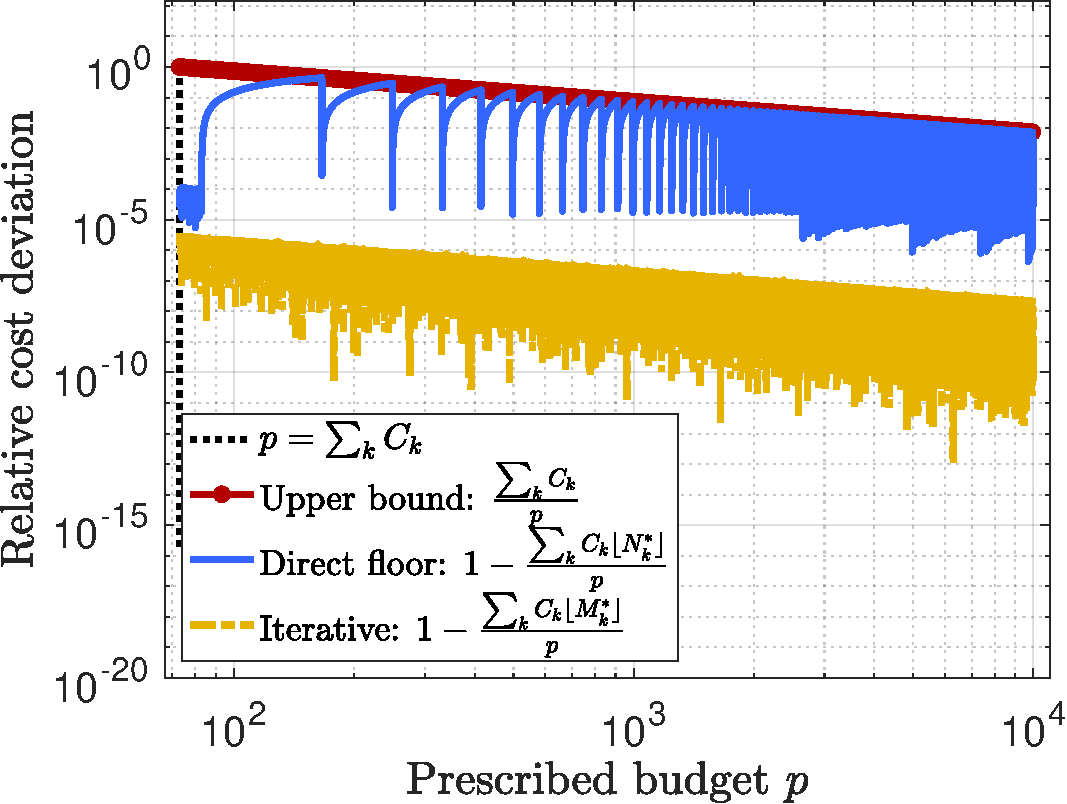
\includegraphics[width=0.45\textwidth]{./Figures/Eg1_Cost.pdf}
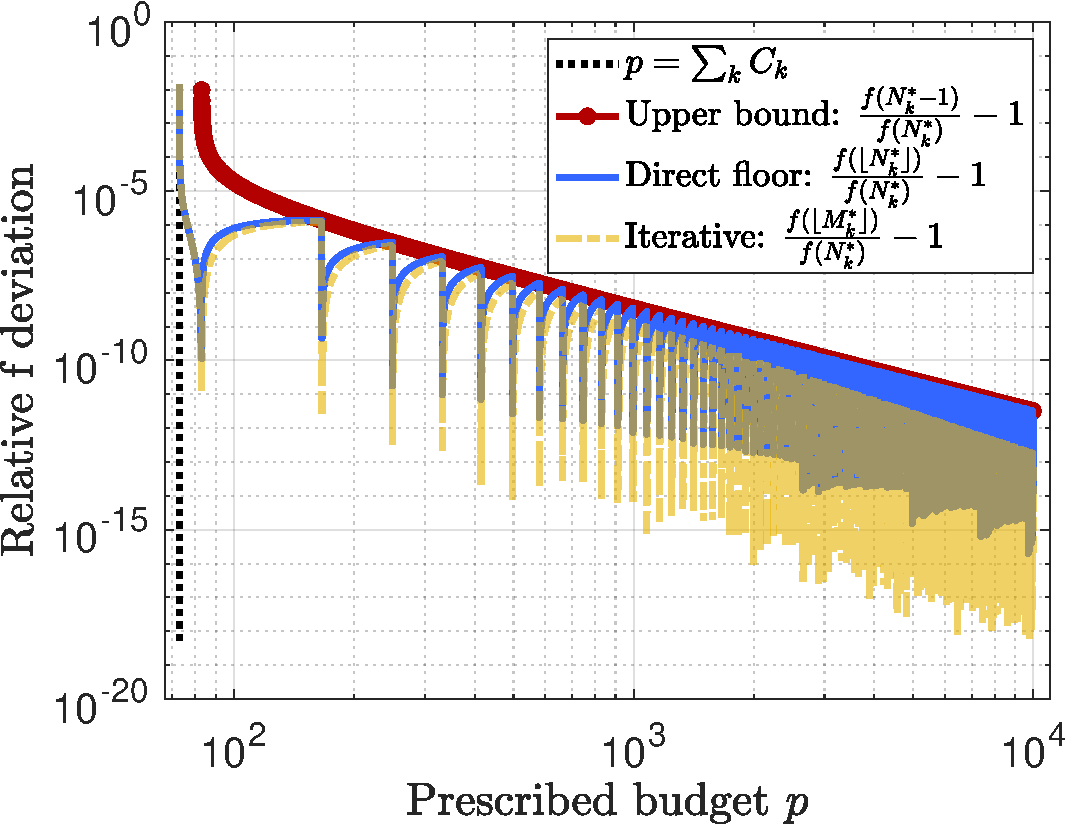
\includegraphics[width=0.45\textwidth]{./Figures/Eg1_f.pdf}
% \caption{Left: Cost deviation vs budget. Right: Variance deviation vs budget.}
\end{figure}

{\footnotesize
\begin{itemize}[leftmargin=15pt] 
\item[$\circ$] Iterative scheme maintains near-zero cost deviation
\item[$\circ$] Characteristic sawtooth patterns from discrete allocations
\item[$\circ$] Consistent variance advantage across budget range
\item[$\circ$] Theoretical bounds validated numerically
\end{itemize}
}
\end{frame}

% ===========================================================
\begin{frame}{Example from Peherstorfer's (p=200)}
\begin{itemize}[leftmargin=5pt] 
\item[$\triangleright$] Data ($p=200$)

\begin{table}[ht]
\centering
\scalebox{0.7}{
\begin{tabular}{|c|c|c|c|c|c|c|}
\hline
Model index &1 &2 &3 &4 \\
\hline
Correlation coeff $\rho_{1,k}$ &1     &9.999882e-01  &9.999743e-01 &9.958253e-01\\
% \hline
% Standard deviation $\sigma_k$ &0.03\\
\hline
Cost &44.395 &6.8409e-01 &2.9937e-01 &1.9908e-04\\
\hline
\end{tabular}
}
\end{table}

\item[$\triangleright$] Result
\begin{table}
\centering
\scalebox{0.7}{
\begin{tabular}{|c|c|c|c|}
\hline
Method & Sample Sizes ($p=200$) & Cost & Variance ($\times 10^{-5}$) \\
\hline
Real-valued & [1.45, 12.68, 330.7, 140360] & 200.00 & 5.0571 \\
Direct floor & [1, 12, 330, 140360] & 179.34 & 5.8074 \\
Iterative & [1, 14, 380, 162080] & 200.00 & 5.3495 \\
\hline
\end{tabular}
}
\end{table}

\item[$\triangleright$] Observations:
{\footnotesize
\begin{itemize}[leftmargin=15pt] 
\item[$\circ$] Iterative maintains advantages: better budget use, lower variance.
\end{itemize}
}
\end{itemize}
\end{frame}


% ===========================================================
\begin{frame}{Budget Sensitivity Analysis}
\begin{figure}
\centering
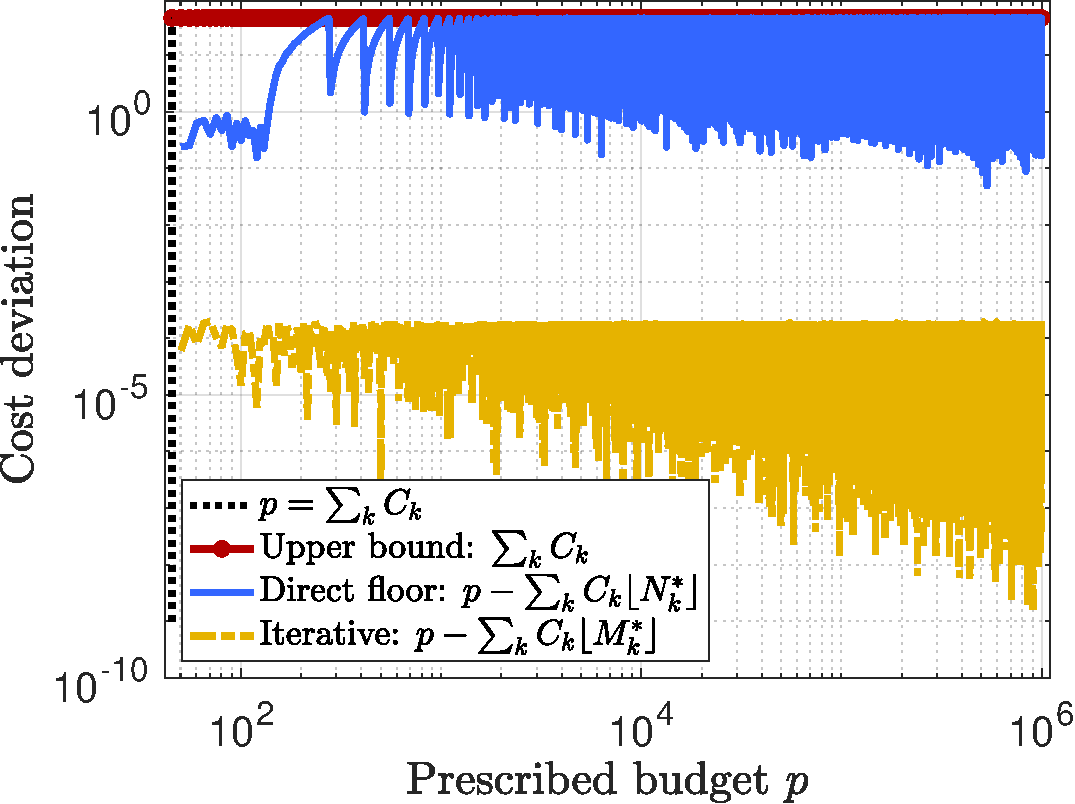
\includegraphics[width=0.45\textwidth]{./Figures/Eg2_Cost.pdf}
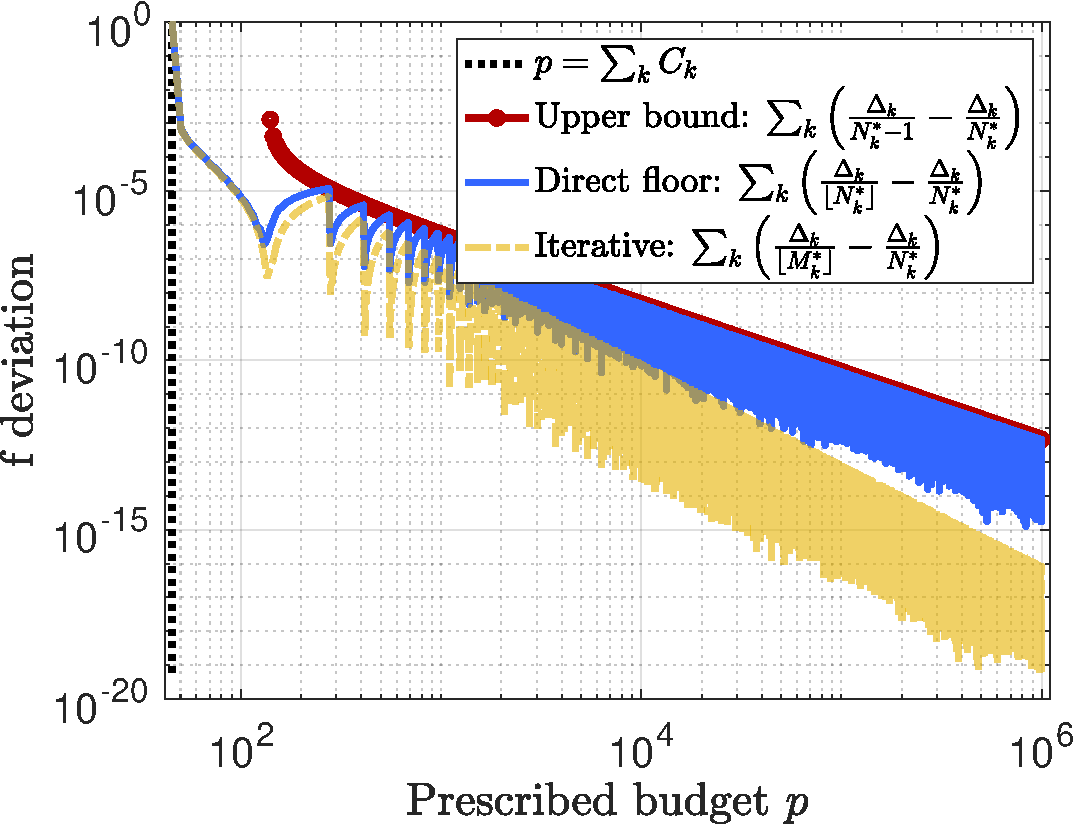
\includegraphics[width=0.45\textwidth]{./Figures/Eg2_f.pdf}
% \caption{Left: Cost deviation vs budget. Right: Variance deviation vs budget.}
\end{figure}

{\footnotesize
\begin{itemize}[leftmargin=15pt] 
\item[$\circ$] Iterative maintains advantages.
\end{itemize}
}
\end{frame}

% % ===========================================================
% \begin{frame}{Modified Allocation for Degenerate Cases}
% \begin{block}{Problem}
% Direct flooring can assign zero samples to high-cost models, causing infinite variance
% \end{block}

% \begin{block}{Solution: Minimum Sample Enforcement}
% \begin{itemize}
% \item Set $\lfloor M_k^* \rfloor = 1$ whenever computed value $< 1$
% \item Redistribute remaining budget iteratively
% \item Preserves estimator feasibility and budget constraint
% \end{itemize}
% \end{block}

% \begin{block}{Results}
% \begin{itemize}
% \item Eliminates degenerate estimators
% % \item 5-7\% variance reduction vs existing modified rounding
% \item Maintains theoretical guarantees
% \end{itemize}
% \end{block}
% \end{frame}



% \begin{frame}{Conclusion}
% \begin{block}{Key Contributions}
% \begin{itemize}
% \item Novel iterative framework for integer MFMC allocation
% \item Dynamic programming formulation with theoretical guarantees
% \item Superior budget utilization and variance performance
% \item Robust handling of degenerate cases
% \item Efficient computational implementation
% \end{itemize}
% \end{block}

% \begin{block}{Future Directions}
% \begin{itemize}
% \item Stochastic programming with uncertain parameters
% \item Adaptive fidelity selection
% \item Multi-information source optimization
% \item Applications to broader resource allocation problems
% \end{itemize}
% \end{block}
% \end{frame}


% % ===========================================================
% \begin{frame}{Numerical Illustration}
% \begin{columns}
% \begin{column}{0.55\textwidth}
% \textbf{Setup:}
% \begin{itemize}
%     \item $K=4$ fidelity levels
%     \item Costs $C_k = [1,\, 0.1,\, 0.01,\, 0.001]$
%     \item Correlations $\rho_{1,k} = [1,\, 0.95,\, 0.9,\, 0.8]$
%     \item Budget $p = 1000$
% \end{itemize}
% \end{column}
% \begin{column}{0.45\textwidth}
% % \includegraphics[width=\textwidth]{variance_cost_curve.pdf}
% \end{column}
% \end{columns}
% \vspace{1ex}
% \centering
% \textbf{Result:} Iterative allocation achieves near-optimal variance and uses full budget.
% \end{frame}



%-----------------------------------------------------------
\begin{frame}
% \frametitle{$|\!\!\sim\! \underline{\hspace{0.25cm}}\!\sim\!\! |@ \underline{\hspace{0.25cm}} @|\!* \!\underline{\hspace{0.25cm}}\!*\!|. \underline{\hspace{0.25cm}} .|- \underline{\hspace{0.25cm}} -|G \underline{\hspace{0.25cm}} G|x\underline{\hspace{0.25cm}} x|/\underline{\hspace{0.25cm}}\backslash|w_w|Q\underline{\hspace{0.25cm}}Q|>\underline{\hspace{0.25cm}}>|=\underline{\hspace{0.25cm}}=|+\underline{\hspace{0.25cm}}+|\#\underline{\hspace{0.25cm}}\#|z\underline{\hspace{0.25cm}}z|>\underline{\hspace{0.25cm}}<|6\underline{\hspace{0.25cm}}9|$}


	\begin{center}
	{\fontsize{35}{70}\selectfont  Thank You $|\neg\underline{\hspace{0.4cm}}\neg|$}
	\end{center}
\end{frame}
%----------------------------------------------------------------



\end{document}